\chapter{Referencial teórico}
Neste capítulo, apresentaremos alguns conceitos e definições teóricas que serão abordadas nesta pesquisa. A \autoref{sec:estudocoorte} apresenta a definição de estudo de coorte e a \autoref{sec:variacoes} apresenta o método de variações idiossincráticas na composição de gênero.

\section{Estudo de coorte}
\label{sec:estudocoorte}
A palavra coorte tem origem no latim \textit{cohors}. Esse termo era utilizado para nomear uma unidade militar do Império Romano, que compunha uma legião. Pode ser considerada equivalente ao conceito moderno de batalhão. No contexto científico, uma coorte pode ser definida como um grupo de pessoas que possuem uma característica ou experiência em comum. Coortes podem ser estabelecidas com vários propósitos. Um deles é a análise de grupos dentro de um determinado domínio, como em estudos econométricos, epidemiológicos e demográficos. Dentro das metodologias utilizadas para explorar uma questão específica estão os estudos observacionais. O que diferencia os estudos de caráter observacional de outros estudos é a realização de intervenções. Nesses estudos, os pesquisadores não interferem nos fenômenos estudados, apenas os observam, fazendo com que a variável considerada não esteja sob controle \autocite{Song2010}.

\begin{figure}[h]
\caption{Tipos de estudos observacionais}
\centering
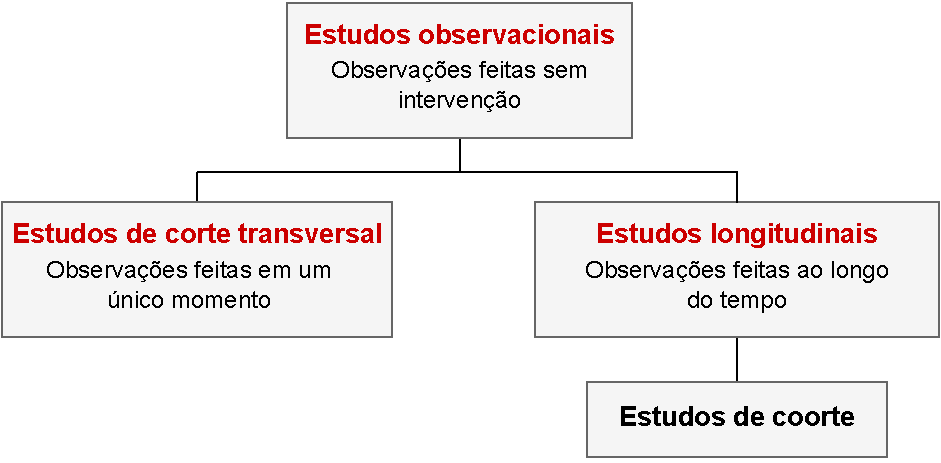
\includegraphics{figuras/Diagrama tipos de estudos observacionais.pdf}
\end{figure}


Estudos observacionais podem ser divididos de acordo com o período de coleta de dados. Quando as observações são feitas em um momento específico, coletando dados em um curto intervalo de tempo, chamamos de estudo de corte transversal. Eles são úteis para observar o estado e as condições atuais dos participantes, sem que haja um acompanhamento dos indivíduos ao longo do tempo \autocite{Zangirolami-Raimundo2018}. 

Já quando os indivíduos são acompanhados por longos períodos de tempo, os estudos são classificados como longitudinais. São realizadas coletas de dados contínuas ou repetidas em intervalos regulares, como dias, meses e anos. Como os dados levam em consideração um grupo pré-definido, é possível ajustar os métodos estatísticos para mudanças observadas ao longo do tempo para o grupo como um todo ou para sujeitos específicos \autocite{Caruana2015}.

Os estudos de coorte são um tipo de estudo longitudinal que leva em consideração uma segmentação específica da população, que é a coorte. Um exemplo de estudo de coorte é a observação do desenvolvimento de doenças em uma população. A amostra populacional pode ser dividida em duas coortes: a coorte 1, de expostos à doença e a coorte 2, de não expostos. Assim, é possível comparar a ocorrência da doença entre os grupos.

Na área da educação, estudos de coorte podem ser utilizados para analisar como questões específicas impactam sujeitos inseridos no sistema educacional, como professores, estudantes e outros envolvidos. \citet{Bjorkenstam993} investigaram a associação do desempenho escolar com taxas de suicídio em estágios posteriores da vida, utilizando uma coorte de nascidos entre 1972 e 1981 na Suécia. Outro exemplo foi o trabalho de \citet{Ensminger1992}, que examinou os caminhos de desenvolvimento de uma coorte de estudantes negros de uma escola de Chicago entre 1966 e 1977. 

A realização de estudos de coorte educacionais, em particular os retrospectivos, como é o atual, é facilitada pela disponibilização de dados públicos de diferentes abrangências. No Brasil, há a inicativa do \href{https://dados.gov.br/home}{Portal Brasileiro de Dados Abertos}, com dados nos níveis federal e local de múltiplas áreas. No sentido desta pesquisa, utilizaremos dados de estudantes que prestaram ENEM em um determinado ano para identificar suas escolas e acompanhá-las ao longo do tempo. Dessa forma, podemos analisar a composição de gênero vis-à-vis outras coortes estudantis.


\section{Estratégias empíricas: Variações idiossincráticas na composição de gênero}
\label{sec:variacoes}
Um desafio na condução de uma pesquisa é isolamento e entendimento do impacto de fatores específicos, como o efeito de pares. O efeito de pares (do inglês \textit{peer effect}) se refere à influência e impactos que indivíduos dentro do círculo próximo (familiar, social ou educacional) têm nas suas decisões e comportamentos. Um trabalho muito relevante no entendimento dos efeitos sociais do grupo que uma pessoa se insere é o de \citet{Manski1993}. Ele aponta a existência de efeitos de pares correlatos, que são comportamentos similares em pessoas do mesmo grupo por conta da semelhança de características individuais ou ambientes institucionais.

Isso é especialmente importante no contexto educacional, já que estudantes do ensino médio compartilham o ambiente escolar durante sua formação. Inseridos em classes diversificadas, eles devem conviver diariamente com outros adolescentes por uma parte relevante de suas vidas. Os colegas de escola podem ser uma importante força social não só no desempenho acadêmico, mas também nas aspirações profissionais e decisões de seguir uma área específica \autocite{Tang2008}.  

A literatura observa que os pares têm grande relevância em comportamentos, escolhas e resultados educacionais \autocite{Sacerdote2014, Zimmerman2003}. Para entender melhor esse efeito, é importante considerar como estão estruturados os grupos de referências de estudantes, já que eles são altamente vulneráveis à influência uns dos outros pela exposição contínua e proximidade. Os efeitos dos pares podem se apresentar tanto de maneira positiva, quanto negativa, que se refletem em pontuações de prova, motivação e hábitos de estudo, por exemplo. 

Manski observa uma dificuldade no isolamento desse efeito no comportamento de uma população. Dentro de um grupo, indivíduos tendem a se relacionar com outros que são parecidos com eles, o que pode dificultar na identificação do efeito real dos pares, já que mudanças comportamentais podem ocorrer tanto devido à influência dos pares, quanto pela associação natural de pessoas com comportamentos similares. Esse indivíduo também pode influenciar o par e por ele ser influenciado simultaneamente. Uma forma de isolar essas influências é através da observação da composição de diferentes coortes ao longo do tempo, isto é, como diferentes distribuições dos pares nas salas de aula afetam os alunos.

Um importante precursor dessas observações é o estudo de \citet{Hoxby-2000}. Ela identificou e mensurou a existência de efeitos dos pares em coortes escolares que diferem na composição de fatores específicos, como o gênero. Nesse sentido, múltiplos trabalhos exploram o problema com uma metodologia similar, denominada de variações idiossincráticas na composição de gênero. Essa estratégia apoia-se na variação aleatória das proporções de estudantes nas coortes escolares. Quando uma característica qualquer é analisada, pode-se ter uma dificuldade na estimativa da regressão por conta da causalidade reversa - variável X influencia váriavel Y -, sem saber qual é a direção da influência. Isso não acontece quando utilizamos a característica de gênero, já que ela é fixa no tempo. Por isso, adotamos a análise do fator de gênero dentro das coortes escolares.

Os modelos econométricos, apesar de semelhantes, diferem por serem estimados utilizando conjuntos de dados educacionais de diferentes países, que se configuram em sistemas de ensino distintos, bem como se apoiam em outros recursos, como registros demográficos. Além disso, podem ser consideradas diferentes etapas da educação básica, como anos iniciais e finais do fundamental e médio. 

Como parte da nossa metodologia se propõe a analisar o efeito da composição de gênero nas escolhas de graduação, utilizaremos como referência o trabalho de \cite{Borges2021}, colaboradora desta pesquisa de mestrado, que se volta para coortes de escolas de ensino médio brasileiras, um contexto similar ao nosso. Para esse propósito, ela emprega dados do Censo Escolar e do vestibular da Universidade Estadual de Campinas (UNICAMP). As definições teóricas apresentadas, assim como a equação definida, foram extraídas do capítulo \textit{Gender peer effects on major choice} \autocite{Borges2021}. 

\subsection{Efeitos de gênero em escolhas de graduação}
Variações idiossincráticas podem ser definidas como particularidades e diferenças individuais únicas que podem influenciar resultados ou comportamentos. Esses fatores comuns ou gerais que afetam um grupo de indivíduos também influenciam os sistemas nos quais estes estão inseridos \autocite{Meister1991}. Essas variações podem ser diversas, abrangendo uma ampla gama de características, experiências e situações pessoais. Alguns exemplos de variações são:

\begin{itemize}
  \item \textbf{Contexto pessoal:} Dinâmica familiar, status socioeconômico, crenças, bagagem cultural, valores familiares;
  \item \textbf{Carreira:} Aspirações e objetivos profissionais, experiência prévia de trabalho, habilidades técnicas; 
  \item \textbf{Educação:} Qualidade escolar, atividades extracurriculares, exposição prematura a tópicos avançados. 
\end{itemize}

Pais e alunos podem escolher suas turmas potenciais, o que pode ser um problema por conta do viés da auto-seleção (\textit{self-selection bias}). Apesar das escolhas pessoais das famílias, utilizamos como hipótese da estratégia empírica que elas não conseguem prever corretamente as variações coorte a coorte na composição de gênero dos estudantes, que seguem processos aleatórios. Assim, explorando a variação idiossincrática de coortes na proporção de alunas, temos um modelo de regressão que estima o impacto de alguns fatores nas variáveis dependentes ($y_{iect}$). No seguinte modelo econométrico, \textit{i} indexa estudante, \textit{e} escolas, \textit{c} coorte e \textit{t} ano do ENEM \footnote{Nesta etapa preliminar, temos dados de apenas um ano (2016). Acrescentaremos outros anos nas etapas subsequentes.}:
\begin{gather*}
y_{iect} = \gamma_0 + \beta_1 \textit{Feminino}_i + \beta_2 \textit{Prop\_FemEM}_{iec} + \\ \beta_3 \textit{Feminino}_i \times \textit{Prop\_FemEM}_{iec} + \alpha_e + \alpha_t + X_i \omega + Z_{ec} \delta + \gamma_{et} + \epsilon_{iect}
\end{gather*}

A equação é composta por:

\begin{itemize}
  \item $\textit{Feminino}_i$, variável binária indicadora de gênero;
  \item $\textit{Prop\_FemEM}_{iec}$, proporção de colegas do gênero feminino na escola \textit{e} no ano de conclusão do ensino médio \textit{c};
  \item $\alpha_e$, efeitos fixos da escola;
  \item $\alpha_t$, efeitos fixos do ano do ENEM;
  \item $X_i$, vetor de características individuais do aluno;
  \item $Z_{ec}$, variáveis da coorte escolar: tamanho da turma, proporção de alunos que frequentam aulas diurnas, idade média dos colegas;
  \item $\gamma_{ec}$, tendência linear de tempo específica da escola;
  \item $\beta_1$, coeficiente de diferenças de gênero nas variáveis de resultados;
  \item $\beta_2$, coeficiente de efeitos de pares de gênero aplicáveis tanto a homens quanto a mulheres;
  \item $\beta_3$, coeficiente do impacto diferencial de mulheres terem uma proporção maior de colegas do sexo feminino;
  \item $\epsilon_{iect}$, clusterização dos erros-padrão.
\end{itemize}

Em todas as estimativas, é realizado um ajuste para a potencial correlação de erros dentro da mesma escola. O conjunto de variáveis de resultado ($y_{iect}$) está relacionado ao objetivo do estudo, que é analisar se a exposição a maiores proporções de colegas do gênero feminino durante o ensino médio afeta as escolhas do curso de graduação. São criadas variáveis binárias para indicar escolha de curso da área STEM e cursos de Tecnologia da Informação (Ciência da Computação e afins).

Utilizaremos metodologia similar à utilizada por \citet{Borges2021} para analisar os efeitos da composição de gênero das coortes de ensino médio nas opções de carreira dos estudantes, dessa vez numa perspectiva mais abrangente, que é proporcionada pelo conjunto de dados do SISU. No próximo capítulo, apresentaremos os trabalhos relacionados, com enfoque naqueles que utilizaram metodologias semelhantes para analisar o efeito da composição de gênero e que se voltam para o cenário brasileiro.